%%% License: Creative Commons Attribution Share Alike 4.0 (see https://creativecommons.org/licenses/by-sa/4.0/)
%%% Slides are based heavily on earlier versions of this course taught by Jesper Rudiger.

\documentclass[english,10pt
%,handout
,aspectratio=169
]{beamer}
%%% License: Creative Commons Attribution Share Alike 4.0 (see https://creativecommons.org/licenses/by-sa/4.0/)
%%% Slides are based heavily on earlier versions of this course taught by Jesper Rudiger and Peter Norman Sorensen.

\DeclareGraphicsExtensions{.eps, .pdf,.png,.jpg,.mps,}
\usetheme{reMedian}
\usepackage{parskip}
\makeatother

\renewcommand{\baselinestretch}{1.1} 

\usepackage{amsmath, amssymb, amsfonts, amsthm}
\usepackage{enumerate}
\usepackage{hyperref}
\usepackage{url}
\usepackage{bbm}
\usepackage{color}

\usepackage{tikz}
\usepackage{tikzscale}
\newcommand*\circled[1]{\tikz[baseline=(char.base)]{
		\node[shape=circle,draw, inner sep=-20pt] (char) {#1};}}
\usetikzlibrary{automata,positioning}
\usetikzlibrary{decorations.pathreplacing}
\usepackage{pgfplots}
\usepgfplotslibrary{fillbetween}
\usepackage{graphicx}

\usepackage{setspace}
%\thinmuskip=1mu
%\medmuskip=1mu 
%\thickmuskip=1mu 


\usecolortheme{default}
\usepackage{verbatim}
\usepackage[normalem]{ulem}

\usepackage{apptools}
\AtAppendix{
	\setbeamertemplate{frame numbering}[none]
}
\usepackage{natbib}




\title{Financial Markets Microstructure \\ Lecture 2}

\subtitle{Prices and Liquidity \\
Chapter 2 of FPR}

\author{Egor Starkov}

\date{K{\o}benhavns Unversitet \\
	Spring 2021}



\begin{document}
	\AtBeginSection[]{
		\frame<beamer>{
			\frametitle{This lecture:}
			\tableofcontents[currentsection,currentsubsection]
	}}
\frame[plain]{\titlepage}
%\addtocounter{framenumber}{-1}


\begin{frame}{What did we do last week?}
	\begin{enumerate}
		\item Introduced \structure{financial markets} broadly speaking and motivate why we wanted to talk about it
		\item Categorize the most important types of \structure{institutions}:  order-driven markets (auctions) and dealer markets
		\item Introduced some of the key \structure{concepts and language}: dealer sets bid/ask price, market/limit order
	\end{enumerate}
\end{frame}


\section{Leftovers: Types of markets and types of agents}

\begin{frame}{Types of Markets: Exchange versus over-the-counter}
	\textbf{Exchange trading}
	\begin{itemize}
		\item Organized exchange venues (NYSE, NASDAQ, LSE, ...)
		\item Generally offer a lot of services
		\begin{itemize}
			\item Liquidity and stability through \textit{specialists/market makers}
			\item Clearing and settlement
			\item Transparency
		\end{itemize}
	\end{itemize}
	\textbf{Over-the-counter (OTC) trading}
	\begin{itemize}
		\item Off-exchange venues
		\begin{itemize}
			\item Use quotation systems to match dealers and traders
			\item However, no guarantee of liquidity (no specialists)...
			\item ...nor transparency: may not publish trade information
		\end{itemize}
	\end{itemize}
	\textbf{Dark liquidity}: Liquidity in `private exchanges' (not public)
\end{frame}


\begin{frame}{Other dimensions}
	\begin{itemize}
		\item Many other aspects in which markets can differ:
		\begin{itemize}
			\item Transparency about current orders
			\item Transparency about past trades
			\item Fragmentation
			\item Listing requirements
			\item ...
		\end{itemize}
		\item Who benefits from markets being organized in a particular way? Who loses? 
	\end{itemize}
\end{frame}


\begin{frame}{Types of players in financial markets}
	\begin{columns}
		\begin{column}{0.4\linewidth}
			\begin{itemize}
				\item \textbf{Traders/investors}: the end-``consumers'' or suppliers of the asset
				\item \textbf{Brokers}: the intermediaries who relay investors' orders to the market (investment banks)
				\item \textbf{Dealers/market-makers}: match orders from different sides of the market
			\end{itemize}
		\end{column}
		\begin{column}{0.6\linewidth}
			\pause[1]
			\includegraphics<handout:0>[scale=0.23]{../L1/pics/ag_brokers}
		\end{column}
	\end{columns}
\end{frame}


\begin{frame}{Types of traders}
	\begin{columns}
		\begin{column}{0.67\linewidth}
			Traders can be classified:
			\begin{itemize}
				\item \structure{Retail investors} vs \structure{institutional investors}
				\begin{itemize}
					\item Retail: regular people, individuals with money.
					\item Institutional: pension funds, mutual funds, hedge funds, private equity funds...
				\end{itemize}
				\item \alert{Informed} vs \alert{uninformed} investors
				\begin{itemize}
					\item Retail investors and pension funds usually have little ``private information''.
					\item Hedge funds and short-selling funds have good analytics and can react fast.
					\item ``Private information''$\neq$``insider information''! Insider trading is banned in most jurisdictions.
				\end{itemize}
			\end{itemize}
		\end{column}
		\begin{column}{0.33\linewidth}
			\pause[1]
			\includegraphics<handout:0>[scale=0.27]{../L1/pics/ag_traders}
		\end{column}
	\end{columns}
\end{frame}



\section{Let's talk about GameStop}

\begin{frame}{GameStop}
	1. What kind of traders are involved on both sides? Based on that fact: why has this story made the news?
\end{frame}


\begin{frame}{GameStop}
	3. Robinhood (trading app) halted trading in GameStop stocks at some point. Is there a scope for some regulatory intervention to prevent this kind of exclusion of retail traders?
\end{frame}


\begin{frame}{GameStop}
	2. Sentiment aside, would now be a good time to buy GameStop stock? Why/why not?
	\pause
	\includegraphics[scale=0.65]{pics/gamestop}
\end{frame}



\section{Fundamental value and Prices}

\begin{frame}{Fundamental Value}
	\begin{itemize}
		\item We'd like to believe there is some ``objective''/``fundamental'' value of a stock.
		\item The previous question then amounts to: \\
		\emph{``Is current price of GME above or below its fundamental value?''}
		\pause
		\item To answer, need to understand what \structure{fundamental value} is.
		\pause
		\item \textbf{Short answer}: \alert{discounted cash flow}. Affected by many factors:
		\begin{enumerate}
			\item R+D
			\item Governance
			\item Marketing
			\item Competition
			\item ...
		\end{enumerate}
	\end{itemize}
\end{frame}


\begin{frame}{Fundamental Value 2}
	\begin{itemize}
		\item Long answer: study \structure{asset pricing}.
		\begin{itemize}
			\item Field of finance devoted to calculating asset price relative to other assets, assuming perfect markets.
		\end{itemize}
		
		\bigskip
		\pause
		
		\item Question of \textbf{market microstructure}: take the `\alert{fundamental value}' as given and analyze how it \alert{translates into prices} in realistic markets.
		\pause
		\begin{itemize}
			\item In GameStop case, divergence due to bubble(?)
			\item Another broad reason for divergence: \structure{limited liquidity}
		\end{itemize}
		
		\pause[2]
		\item Dual question: \structure{price discovery} \\
		\emph{``How much information about the fundamental value can be extracted from market prices?''}
	\end{itemize}
\end{frame}



\section{Liquidity}

\begin{frame}{What is liquidity?}
	\begin{itemize}
		\begin{columns}
			\begin{column}{0.7\linewidth}
				\item In \structure{perfect markets}:
				\begin{itemize}
					\item There is one price = valuation cutoff
					\item Agents who value asset above the cutoff end up with it (keep or buy)
					\item Agents who value asset less end up without it (sell or do not buy)
					\item This is the \alert{efficient} allocation that we want
				\end{itemize}
				\pause
				\item In \structure{real markets}:
				\begin{itemize}
					\item Bid/ask prices different from that ideal cutoff/fundamental value
					\item (due to limited liquidity)
					\item Allocation \alert{inefficient}
				\end{itemize}
				\vspace{2em}
				% liq = distance from perfect market / degree of perfection
			\end{column}
			\begin{column}{0.3\linewidth}
				\pause[1]
				\includegraphics<1>[scale=0.23]{pics/L2_prices1.png}%
				\includegraphics<2->[scale=0.23]{pics/L2_prices2.png}
				\vspace{-3em}
			\end{column}
		\end{columns}
		
	\end{itemize}
\end{frame}


\begin{frame}{Still, what exactly is liquidity?}
\begin{itemize}
	\item \alert{Market liquidity} = \visible<handout:0>{``market's ability to facilitate an asset being sold quickly without having to reduce its price very much (or even at all)''}
	\visible<handout:0>{
		\begin{itemize}
			\item Not everyone who wants to trade in a given asset is present in the market at the same time
		\end{itemize}
	}
	\pause
	\item Do not confuse with (related notions of):
\end{itemize}
\begin{enumerate}
	\item \structure{Funding liquidity} = \visible<handout:0>{``economic agent's ability to obtain cash/credit at acceptable terms, to meet obligations without incurring large losses''}
	\visible<handout:0>{
		\begin{itemize}
			\item Banks are `liquidity constrained' when they do not have enough cash on hands to meet demand for withdrawals (despite having enough assets)
			\item You are liquidity constrained when your wage arrives in two days but you need to pay your rent today.
		\end{itemize}
	}
	\item \structure{Monetary liquidity} = \visible<handout:0>{``asset's ability to be exchanged for goods''}
	\visible<handout:0>{
		\begin{itemize}
			\item Assets in the order of decreasing liquidity: cash, checking deposits, long-term deposits, housing, ...
		\end{itemize}
	}
\end{enumerate}
\end{frame}


\begin{frame}{Why do we care about liquidity?}
\begin{itemize}
	\item Traders: liquidity provides a measure of trading costs
	\item Regulators:
	\begin{enumerate}
		\item Efficiency is tricky to measure in financial markets: liquidity provides a proxy
		\item Illiquid markets also seem to be more prone to medium-run price deviations from fundamentals
		\item Illiquidity \textit{may} be a sign of structural problems in the market
	\end{enumerate}
	\item Relation to \structure{depth}: depth measures how much must be traded to move price by certain amount
	\begin{itemize}
		\item $\approx$ sensitivity of liquidity to trade size
	\end{itemize}
\end{itemize}
\end{frame}


\begin{frame}{Liquidity dry ups}
	Liquidity can change over time, can dry up in times of instability
	\begin{center}
		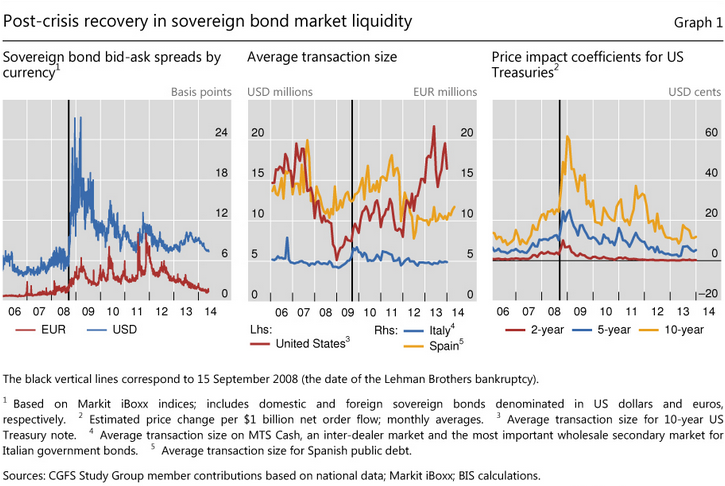
\includegraphics[scale=0.5]{pics/L2_liquiditylehman}
	\end{center}
\end{frame}



\section{Measures of Liquidity}

\begin{frame}<handout:0>{Liquidity measures}
There is not a unique measure of liquidity. We will consider several:
\begin{enumerate}
	\item \textbf{Spread measures}: quoted spread, effective spread, realized spread
	\item \textbf{Volume-weighted average price}: simply using average prices
	\item \textbf{Price impact}: How much does the price move after a trade
	\item \textbf{Non-trading measures}: trading volumes
\end{enumerate}

When trade direction is not available: estimate via \structure{Lee-Ready algorithm}. 

When quote data are not available: estimate them using \structure{Roll's measure}
\end{frame}


\begin{frame}<handout:0>{Example}
	\begin{itemize}
		\item We will play around with a dataset on KrispyKreme stock
		\begin{center}
			%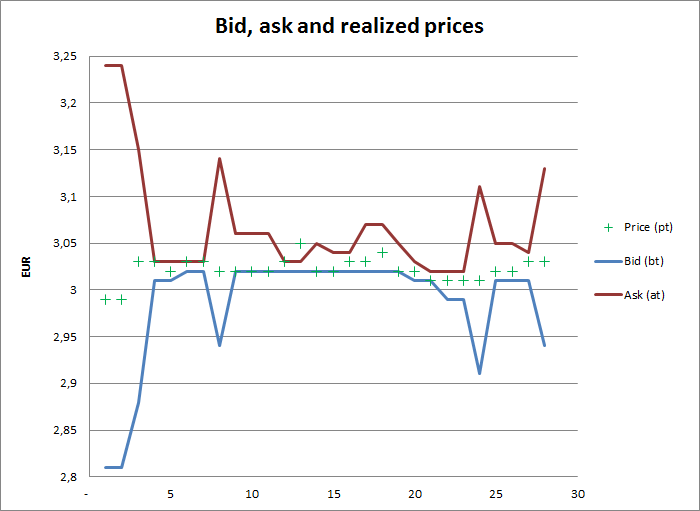
\includegraphics[scale=0.34]{pics/L2_bidask}
			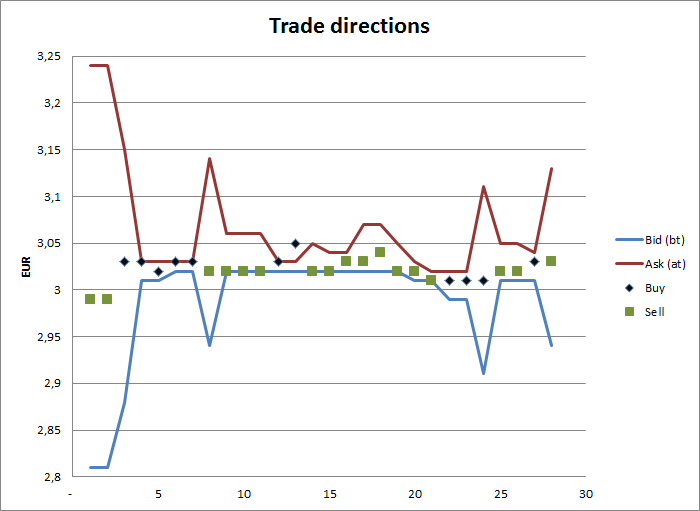
\includegraphics[scale=0.34]{pics/L2_directions}
		\end{center}
		\pause
		\item Notice that price is sometimes inside spread\visible<handout:0>{: price improvements (either hidden limit orders or price improvement given by dealer)}
		\item Also a price outside spread\visible<handout:0>{ (recall bid/ask only valid for x units)}
	\end{itemize}
\end{frame}


\begin{frame}{Quoted spread}
	\begin{itemize}
		\item Let $a_t$ ($b_t$) be the best ask (bid) price at time $t$
		\item \alert{Quoted spread}:
		\begin{equation*}
			S_t = a_t -b_t
		\end{equation*}
		\item Contemporaneous: spread facing trader at time $t$
		\item \pause Normalize to get \alert{normalized quoted spread}
		\begin{center}
			$
			s_t = \frac{S_t}{m_t},
			$
		\end{center}
		where $m_t$ is the midprice:
		\begin{center}
			$
			m_t = \frac{a_t+b_t}{2}.
			$
		\end{center}
		\pause
		\item We can generalize it to consider average spread for trade size $q$: 
		\begin{center}$S_t(q)=\overline{a}_t(q)-\overline{b}_t(q)$\end{center}
		where $\overline{a}_t(q)$ and $\overline{b}_t(q)$ are average execution prices
	\end{itemize}
\end{frame}


\begin{frame}<handout:0>{Quoted spread}
	\begin{itemize}
		\item Applying the definition to the data, we get:
		\begin{center}	
			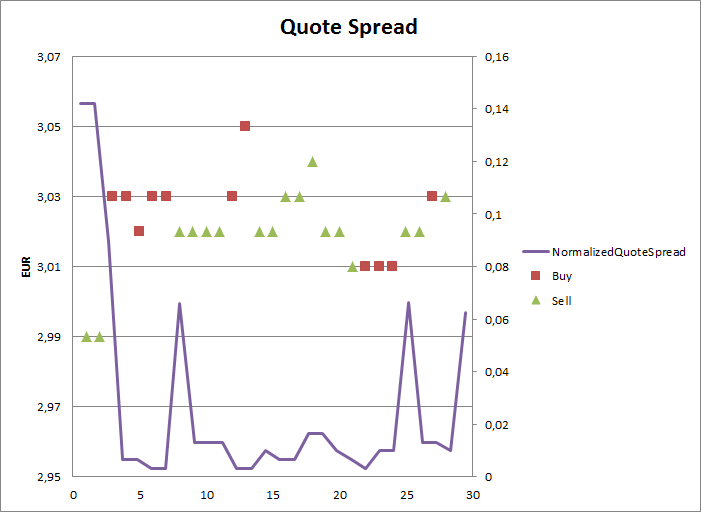
\includegraphics[scale=0.35]{pics/L2_quotespread}
		\end{center}
		\item Notice that the quoted spread does not capture price improvements (for instance in the first three observations)
	\end{itemize}
\end{frame}


\begin{frame}{Effective spread}
	\begin{itemize}
		\item Suppose one market order is executed per period, and
		\begin{itemize}
			\item $d_t$: trade direction (1: buyer-initiated, -1: seller initiated)
			\item $p_t$:  price
		\end{itemize}
		\item \alert{Effective (half-)spread}: 
		\begin{align*}
		S^e_t & = d_t(p_t-m_{t}), \\
		s^e_t & = \frac{S^e_t}{m_{t}}
		\end{align*}
		\item Backward looking: spread faced by previous trader
		\item Compare actual price with midquote the instant before: measures price impact and captures `price improvements'
	\end{itemize}
\end{frame}


\begin{frame}<handout:0>{Effective spread}
	\begin{itemize}
		\item Apply to data and compare to quoted spread
		\begin{center}
			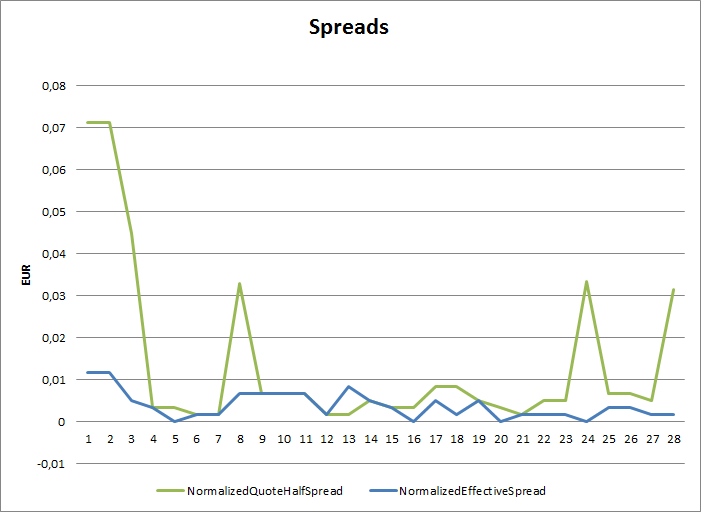
\includegraphics[scale=0.39]{pics/L2_effectivespread}
		\end{center}
		\item Effective spread is often lower (since it captures price improvements)
	\end{itemize}
	% effective and quoted spreads measure cost of trading for the trader
\end{frame}


\begin{frame}{Realized spread}
	\begin{itemize}
		\item \alert{Realized spread}:
		\begin{align*}
		S^r_t & = d_t(p_t - m_{t+\Delta}) \\
		& = d_t(p_t-m_t) - d_t(m_{t+\Delta}-m_t)
		\end{align*}
		\item Spread realized by somebody who holds the asset for $\Delta$ periods
		% ...like a dealer
		\item Idea: measure the spread after prices have adjusted to new information
		\item As a forward-looking measure:
		\begin{itemize}
			\item $\mathbb{E}_t S_t^r = d_t(p_t - m_t) = S_t^e$ if $\mathbb{E}_t m_{t+\Delta} = m_t$
		\end{itemize}
		\item As a backward-looking measure:
		\begin{itemize}
			\item Typically smaller than effective spread: why?
		\end{itemize}
	\end{itemize}
\end{frame}


\begin{frame}<handout:0>{Realized spread}
	\begin{itemize}
		\item Calculate for $\Delta=5$ and compare to other measures
		\begin{center}
			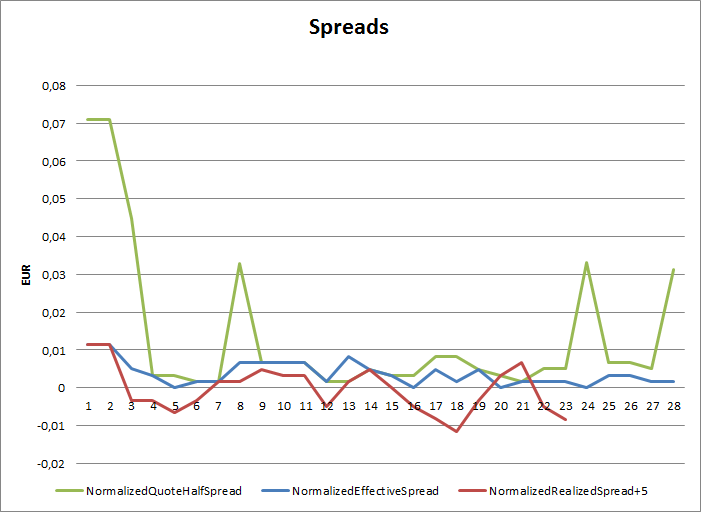
\includegraphics[scale=0.39]{pics/L2_realizedspread}
		\end{center}
		\item Realized spread is indeed often lower than effective spread
	\end{itemize}
\end{frame}


\begin{frame}{Comparing the spreads}
	\begin{itemize}
		\item The \structure{quoted spread} and the \structure{effective spread} may be more useful to traders:
		\begin{itemize}
			\item Quoted spread: what is the quoted trading cost now 
			\item Effective spread: what was the trading cost faced by the last trader
		\end{itemize}
		These are (imperfect) measures of the cost of executing a market order now
		\item The \structure{realized spread} is more relevant to a market maker (liquidity provider):
		\begin{itemize}
			\item It measures the cost of taking a position (long or short) for an amount of time
		\end{itemize}
	\end{itemize}
\end{frame}



\section{Estimating Direction of Trade}


\begin{frame}{Estimating direction of trade}
	\begin{itemize}
		\item We often only observe quotes and realized prices: not the direction of trade
		\item Thus, we need to develop methods to classify trades
		\item Complication: trading may be `within the quotes': harder to guess direction
		\item \alert{Lee-Ready algorithm}: (\citet{lee_inferring_1991})
		\[
		d_t = \left\{
		\begin{aligned}
		1 & \text{ if } |p_t-a_t| < |p_t-b_t| \\
		&\text{ or } p_t=m_t \text{ and } p_t>p_{t-1}\\
		-1 & \text{ if } |p_t-a_t| > |p_t-b_t| \\
		& \text{ or } p_t=m_t \text{ and } p_t<p_{t-1} \\
		\end{aligned}
		\right.
		\]
	\end{itemize}
\end{frame}


\begin{frame}<handout:0>{Estimating Lee-Ready}
	First, we calculate midprices and compare to trade prices
	\center
	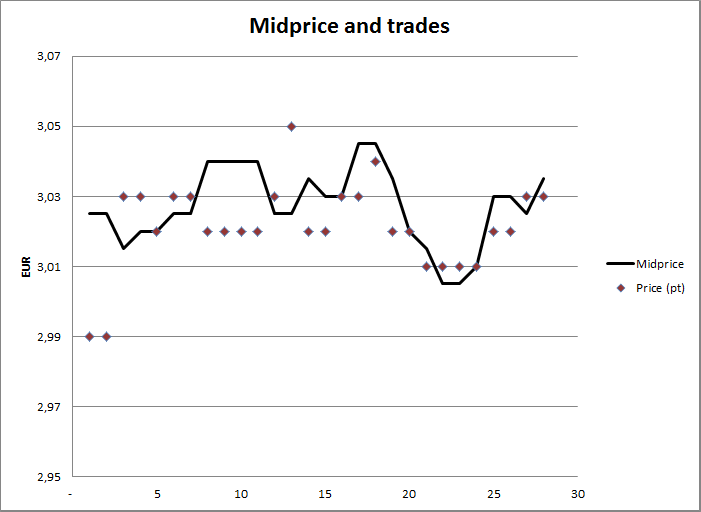
\includegraphics[scale=0.39]{pics/L2_midandtrade}
\end{frame}


\begin{frame}<handout:0>{Estimating Lee-Ready (2)}
	Then we compare trade prices to midprices
	\center
	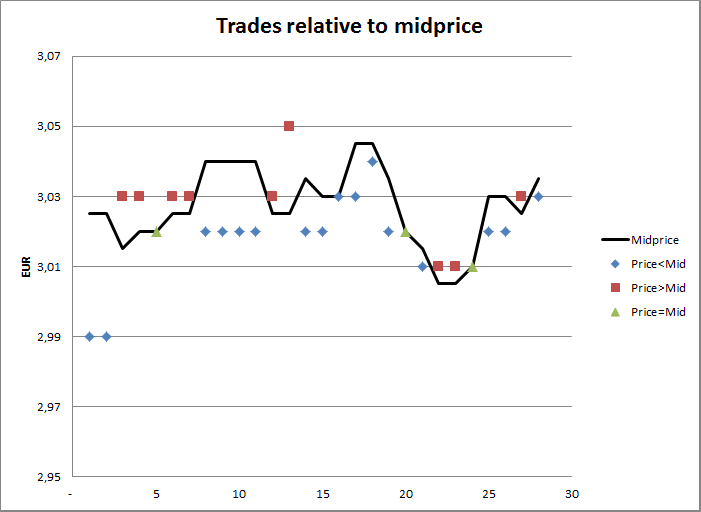
\includegraphics[scale=0.39]{pics/L2_traderelativemid}
\end{frame}


\begin{frame}<handout:0>{Estimating Lee-Ready (3)}
	Finally, we classify the trades that were just on the midprice
	\center
	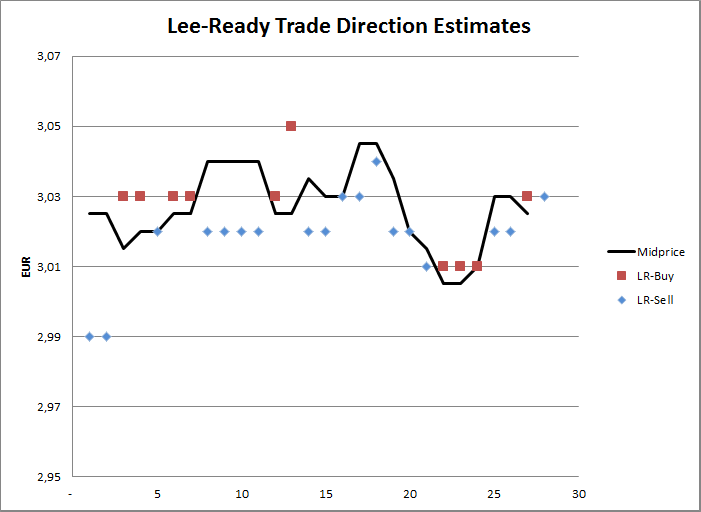
\includegraphics[scale=0.39]{pics/L2_leereadyest}
	% the second tie is ambiguous. look at m_{t+1} vs m_t?
\end{frame}


\begin{frame}<handout:0>{Estimating Lee-Ready (4)}
	Checking with the actual trade directions, we see that we only made one mistake
	\center
	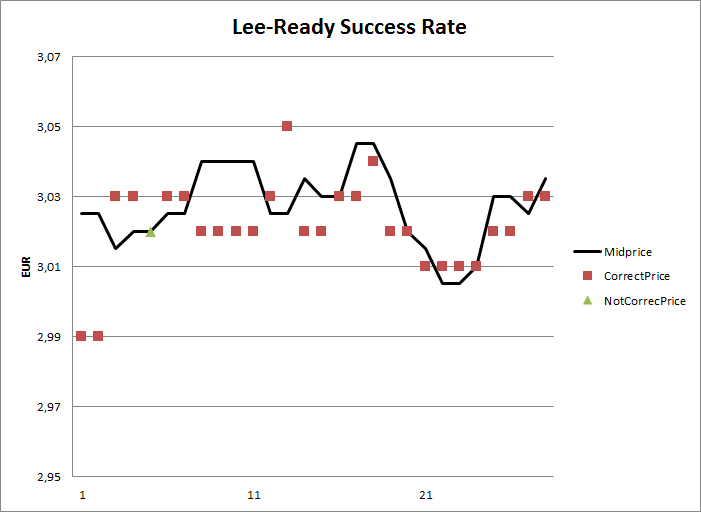
\includegraphics[scale=0.39]{pics/L2_leereadysuccess}
\end{frame}


\begin{frame}{Lee-Ready precision}
	\begin{itemize}
		\item \citet{odders-white_occurrence_2000}: large-scale ($>400$k transactions) test of Lee-Ready algorithm with NYSE data
		\item 85\% correct
		\item Most mistakes with:
		\begin{itemize}
			\item trades at the midpoint
			\item small transactions
			\item transactions in large-cap / frequently traded stocks
			\item (why?)
		\end{itemize}
	\end{itemize}
\end{frame}



\section{Estimating Quotes}


\begin{frame}{Quote data}
	\begin{itemize}
		\item We often lack information on quotes to compute the spread
		\begin{itemize}
			\item Can we estimate the spread knowing only trade prices?
		\end{itemize}
		\item \citet{roll_simple_1984}: use transaction prices to estimate it
		\begin{enumerate}
			\item Construct a simple model of trading and calculate spread
			\item Estimate it
			\item Check robustness to simplifying assumptions
		\end{enumerate}
		%\item Roll's estimator can almost always be computed
	\end{itemize}
\end{frame}


\begin{frame}{Roll's model}
	Suppose the following:
	\begin{enumerate}
		\item All trades have the same size. $d=1$: buy, $d=-1$: sell
		\item Arriving orders are i.i.d. with $\mathbb{P}(d_t =1)=\frac{1}{2}$
		\item Midquote is random walk: $m_t = m_{t-1} + \epsilon_t$  , where $\epsilon_t$ are i.i.d. shocks
		\item Market orders are not informative: $\mathbb{E}(d_t \epsilon_t)=\mathbb{E}(d_t \epsilon_{t+1})=0$
		\item Spread $S = a_t-b_t$ is constant.
	\end{enumerate}
	Then
	\[
	p_t = m_t + \frac{d_t S}{2}.
	\]
	We know $p_t$ but not $m_t$. How do we estimate $S$?
\end{frame}


\begin{frame}{Roll's model}
	\begin{itemize}
		\item Roll's observed that although $\epsilon_t$ and $d_t$ are i.i.d., $\Delta d_t = d_t - d_{t-1}$ is mean-reverting:
		\begin{align*}
			Cov(\Delta d_t, \Delta d_{t-1})	&= -1
			\\
			\pause[2]
			\visible<handout:0|+->{\Rightarrow Cov(\Delta p_t, \Delta p_{t-1}) &= Cov(p_t-p_{t-1}, p_{t-1}-p_{t-2})}
			\\
			\visible<handout:0|+->{&=Cov \left( \frac{S}{2}d_t - \frac{S}{2}d_{t-1} + \epsilon_t, \frac{S}{2}d_{t-1} - \frac{S}{2}d_{t-2} + \epsilon_{t-1} \right)}
			\\
			\visible<handout:0|+->{&= \frac{S^2}{4} Cov \left( d_t-d_{t-1}, d_{t-1}-d_{t-2} \right)}
			\\
			\visible<handout:0|+->{&= \frac{S^2}{4} \mathbb{E}[( d_t-d_{t-1})(d_{t-1}-d_{t-2})]}
			\\
			\visible<handout:0|+->{&= \frac{S^2}{4} \mathbb{E} [-d_{t-1}^2] = \frac{-S^2}{4}}
		\end{align*}
		\item Intuitively: $\Delta d_t>0$ means that we go from a sale to a buy - the next change must be opposite
	\end{itemize}
\end{frame}


\begin{frame}{The estimator}
	\begin{itemize}
		\item We can then work out that
		\[
		Cov(\Delta p_t, \Delta p_{t-1}) = - \frac{S^2}{4},
		\]
		giving us the estimator
		\[
		S^R_t = 2 \sqrt{-Cov(\Delta p_t, \Delta p_{t-1})}.
		\]
		\item Recall the assumptions of the model. We (the book) can work out extensions to treat some of them
		\item In our example: $S^R_t = 0.01$
		%\item Which of the previous spreads is Roll's estimator closest to? % ???
	\end{itemize}
\end{frame}


\section{Other Measures of Liquidity}


\begin{frame}{Price impact}
\begin{itemize}
	\item How much do trades affect prices? \alert{Price impact} $\lambda$;  $1/\lambda$ captures market \textit{depth}
	\[
	\Delta m_t = \lambda q_t + \epsilon_t.
	\]
	Here $q_t$ is the \structure{order imbalance} in period $t$. 	
	In our example: $\lambda = 0.15 $ ($q_t$ in 100,000EUR)
	
	\pause
	\item \alert{Hasbrouck measure} ($\gamma$): sensitivity of returns to trading volume (\citet{hasbrouck_empirical_2007})
	\[
	|\Delta m_t | = \gamma Vol_t + \epsilon_t.
	\]
	In our example: $\gamma = 0.01$ ($Vol_t$ in 100,000EUR)
	
	\pause
	\item \alert{Amihud measure} ($I_t$): take ratio btw return $\Delta m_t$ and volume to get \textit{illiquidity ratio}: (\citet{amihud_illiquidity_2002})
	\center
	$I_t = \frac{|\Delta m_t|}{Vol_t}$.
	%$I_t = \frac{|r_t|}{Vol_t}$.
\end{itemize}
\end{frame}


\begin{frame}<handout:0>{Amihud's Illiquidity Ratio}
\begin{center}
	\includegraphics[scale=0.39]{pics/L2_Amihud}
\end{center}
Somewhat volatile on high-frequency data, usually taken as an average over longer intervals (month)
\end{frame}


\begin{frame}{Volume based measure}
\begin{itemize}
	%\item Let $q_t$ be the order imbalance (net market purchase)
	% volumes or imbalances?
	\item \alert{Volume-Weighted Average Price} (VWAP):
	\[
	VWAP = \sum  w_i p_i,
	\]
	where $w_t = |q_i|/\sum_i |q_i|$ is the order weight, $q_i$ is the size of order $i$
	\item This equals the amount of dollars traded over the number of shares traded: average price
	\item Trader can compare the price he got with VWAP to evaluate how good was his deal relative to market.
	\item This measure may depend excessively on few orders (if they are large) and therefore be subject to manipulation
	\item For our example, $VWAP=3.02$
\end{itemize}
\end{frame}


\begin{frame}{Implementation shortfall}
	\begin{itemize}
		%\item The previous measures the time it takes to execute order %TODO - ???
		\item Aim at time 0: to (net) purchase $q$ shares
		\begin{itemize}
			\item By time $t$, fraction $\kappa_t$ has been executed, at an average execution price $\bar{p}_t$
			\item The realized trading gain is $\kappa_t q(m_t-\bar{p}_t)$
			\item An ideal gain from immediate execution without price impact would have been $q(m_t - m_0)$
			\item The difference is the \alert{implementation shortfall}:
			\begin{align*}
			IS_t 
			& = q(m_t-m_0) - \kappa_t q (m_t - \bar{p}_t) \\
			& = \kappa_t q(\bar{p}_t - m_0) + (1-\kappa_t) q (m_t - m_0).
			\end{align*}
			\item Interpretation: Execution cost plus opportunity cost
		\end{itemize}
	\end{itemize}
\end{frame}


\begin{frame}<handout:0>{Implementation shortfall}
	\begin{itemize}
		\item Suppose in the KrispyKreme example you want to buy 3,500 shares
		\item And suppose all the buy orders in the data (3,400 shares) came from you
	\end{itemize}
	\center
	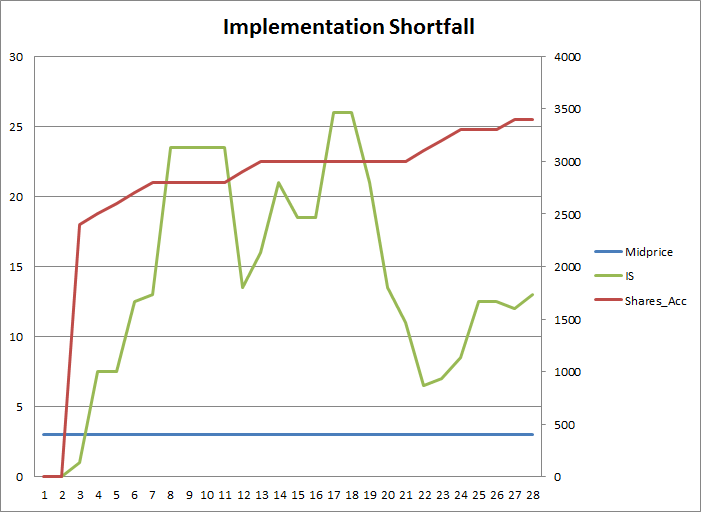
\includegraphics[scale=0.39]{pics/L2_is}
\end{frame}


\begin{frame}<handout:0>{Implementation shortfall}
	Breaking down the shortfall into opportunity cost and execution cost
	\center
	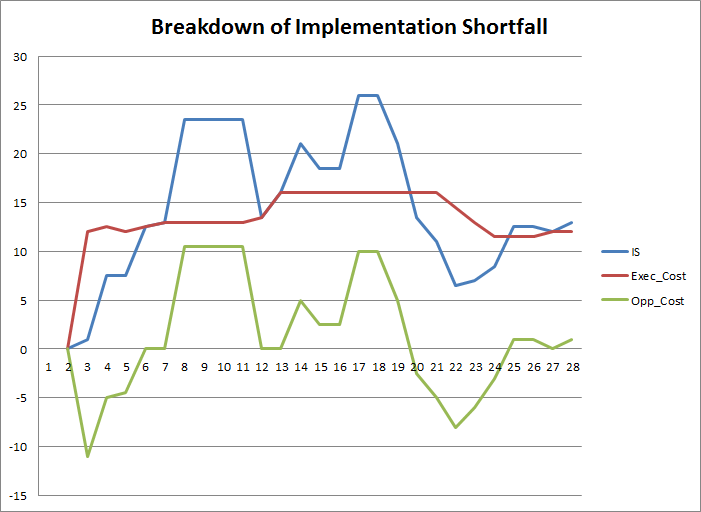
\includegraphics[scale=0.39]{pics/L2_is2}
\end{frame}


\begin{frame}{Other measures}
\begin{itemize}
	\item Measures such as trading volume and trade frequency are also used
	\item Some measures may contradict each other, e.g.:
	\begin{itemize}
		\item trading volume and spreads are both positively correlated with information releases (why?)
		\item price volatility is low in very liquid -- but also very illiquid markets
	\end{itemize}
	\item Frequency of trading or related measures may be more relevant in `thin' markets, for instance in emerging economies
\end{itemize}
\end{frame}


\begin{frame}{Conclusion}
	\begin{itemize}
		\item We have looked at different manners in which to estimate liquidity
		\item No method is perfect: depends on trade size, time horizon, trade motivation
		\item Data shows that liquidity varies both continuously throughout a trading day, and more abruptly around big events
		\item Next time we will start analyzing \textit{what} drives the spread
	\end{itemize}
\end{frame}


\begin{frame}{Exercises for next week}
	\begin{itemize}
		%\item In Absalon, I have attached a commission and fee schedule from Robinhood Financial. More information on \url{www.robinhood.io/}. Discuss the potential effect on other brokerage services.
		%\item In this course we mostly imply equity markets. Read the article (on Absalon) about corporate bond markets. Discuss how differences in market structures of stock and bond markets affect liquidity in these markets.
		\item Recreate the graphs and figures and numbers I presented today using the KrispyKreme dataset
		\item Solve exercise 8 regarding implementation shortfall, on page 75 in the textbook.
		Discuss the meaning of $m_t$ in this analysis.
	\end{itemize}
\end{frame}




\appendix
\begin{frame}[allowframebreaks]{References}
	\bibliography{../teaching}
	\bibliographystyle{abbrvnat}
\end{frame}


\end{document} 







%\begin{frame}{Trade and Prices}
%	\begin{itemize}
%		\item Price theory is fundamental to economics
%		\begin{itemize}
%			\item Law of one price; no arbitrage
%		\end{itemize}
%		\item In financial markets: often a \textit{bid} and an \textit{ask} price. The difference between the two is called the `\textbf{bid-ask spread}'
%		\begin{itemize}
%			\item We will spend time analyzing what drives this spread
%		\end{itemize}
%	\end{itemize}
%\end{frame}
%
%
%\begin{frame}{Market Liquidity}
%	\begin{itemize}
%		\item So far, you have been used to analyzing (long-run) equilibrium allocations and prices
%		\item In practice, prices adjust to temporary imbalances
%		\begin{itemize}
%			\item Not everyone who wants to trade in a given asset is present in the market at the same time
%			\item Example: too many sellers $\rightarrow$ prices lower in short run
%			\item Example: costly to execute large order quickly
%		\end{itemize}
%		\pause
%		\item These effects are related to the \textbf{liquidity} of the asset
%		\begin{itemize}
%			\item Wikipedia: `market liquidity' is a market's ability to facilitate an asset being sold quickly without having to reduce its price very much
%			\item Easy to sell a Google stock (many potential buyers), but maybe hard for a stock of a small Danish company
%		\end{itemize}
%		\item We will develop measures of liquidity in this course
%		\item More liquid assets may be more valuable
%	\end{itemize}
%\end{frame}
